\subsection{Spike Encoders}


Understanding how to translate typical data, such as pixel values from images or scalar values, into spike trains is key to working with neural models. Spike trains, which are sequences of neuron firing activities, act as a sort of language that these models use to handle and process information. 

In this section, we will discuss some of the common methods used to encode this kind of data into spike trains. Each method has its own approach to the transformation and is suited for different types of data or applications. We aim to provide a clear overview of these encoding strategies, exploring how they work, their advantages and drawbacks, and where they can best be applied.


\subsection{Rate Encoding}

Lets try and see how to to encode Mnist digit data set via Rate Encoding specified in \ref{ssec:rate-encoding}.

By using equation \ref{eq:rate-enc-prob}, we can implement the rate encoding approach in a way that controls the spike generation based on the input image and ensures that high-intensity pixels (corresponding to higher values of \(f(x_{i,j})\)) will appear in more patterns.

Overall, the rate encoding approach, combined with the derived probability constraints and stochastic spike generation, enables us to effectively convert an image into a time-varying sequence of spikes while preserving its features. This method allows us to model the behavior of real neurons and capture the temporal dynamics of the input information, making it suitable for various applications in neural information processing and spiking neural network simulations.

\begin{figure}[H]
    \centering
    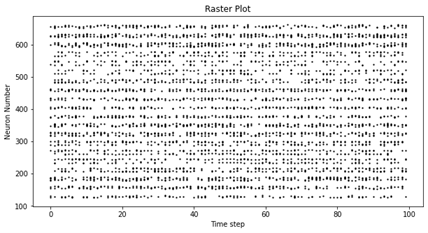
\includegraphics[width=0.5\textwidth]{methods/spike-encoding/graphs/rate-encoding-raster.png}
    \caption{Raster plot of a random Mnist image encoded via Rate Encoding with maximum rate of 20 Hz over trial time of 1 sec}
    \label{fig:rate-encoding-raster}
\end{figure}


\subsection{Latency Encoding}

\textbf{Latency Encoding:}

Implementing Latency Encoding (see \ref{ssec:latency-encoding}) on the MNIST digits dataset presents a challenge. Specifically, the distribution of pixel intensity values within each image poses a substantial difficulty.

\begin{figure}[H]
    \centering
    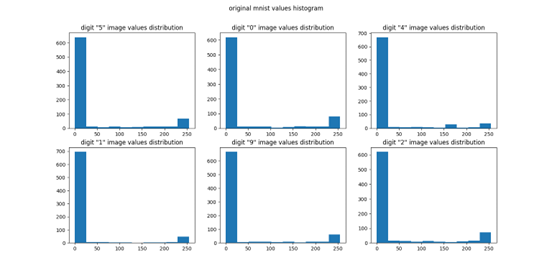
\includegraphics[width=0.8\textwidth]{methods/spike-encoding/graphs/mnist-values-histogram.png}
    \caption{histograms of the pixel values of random Mnist images divided into 10 bins}
    \label{fig:mnist-values-histogram}
\end{figure}

Although having many zero values is not a problem and can even help with achieving sparsity, we face difficulties with the distribution of non-zero values. They are often clustered around two or three key values. This becomes problematic when using linear normalization with logarithmic encoding, which is not effective in distinguishing closely situated values.

This problem is clearly depicted in the raster plot of the encoding:


\begin{figure}[H]
    \centering
    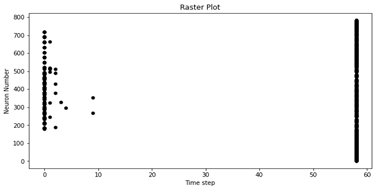
\includegraphics[width=0.8\linewidth]{methods/spike-encoding/graphs/latency-encoding-raster.png}
    \caption{raster plot of a random Mnist image encoded via latency encoding}
    \label{fig:latency-encoding-raster}
\end{figure}

To fix it, we suggest linear latency encoding by:
\begin{equation}
t(I_{\text{in}}) = -\tau \cdot \left(R \cdot I_{\text{in}} - V_{\text{thr}}\right)
\end{equation}

And clipping the zero values (they hold no useful information). The green lines represent the $\tau$ value, and the red lines represent $v_{\text{thr}}$.

\begin{figure}[H]
    \centering
    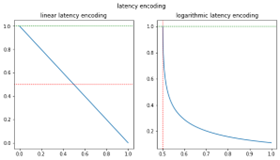
\includegraphics[width=0.5\linewidth]{methods/spike-encoding/graphs/exp-to-linear.png}
    \caption{on the right - the exponential latency encoding function, on the left - the liner latency encoding function}
    \label{fig:latency-exp-vs-lin}
\end{figure}

And as we can see, the results are significantly improved:

\begin{figure}[H]
    \centering
    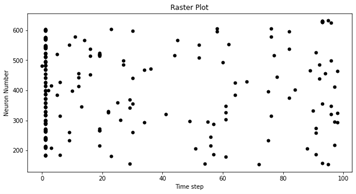
\includegraphics[width=0.7\linewidth]{methods/spike-encoding/graphs/latency-encoding-raster-linear.png}
    \caption{ raster plot of a random Mnist image encoded via linear latency encoding}
    \label{fig:latency-encoding-raster-linear}
\end{figure}

\subsection{Population Encoding}

We shall now delve into various strategies to adopt the population encoding method. Our focus is to utilize this approach in a manner that leverages the salient features of the data, harnesses the unique characteristics of the neuron model, and employs the diverse encoding methodologies we have previously explored in \ref{ch:computational-models}.

As we discussed in section \ref{ch:computational-models}, we can integrate different Spike Encoding functions to extract the features we want.

In Statement \ref{st:window-width}, we demonstrated that each spike response has a distinct temporal extent. This 'window' signifies the period during which the spike can affect the downstream, or afferent, neurons it is connected to.

From the perspective of an efferent neuron, the duration for assessing the afferent spike rate is crucial for accurate interpretation. Assuming the spike generation obeys a Poisson distribution, the confidence interval for the actual coded frequency, $F$, can be evaluated based on the observed frequency, $f = \frac{\text{spikes}}{\Delta T}$. A limited evaluation time, $\Delta T$, potentially introduces inaccuracies in this process. The degree of such inaccuracies directly influences the fidelity of information transmission across the network.

The significance of neural activity is not just about whether spikes occur but also how frequently they occur. Accordingly, it's crucial for our models to interpret these spike rates in order to make informed decisions.

When the assessment duration is short, the observed spike frequency may not accurately represent the true spike rate due to the inherent stochastic nature of spike generation, leading to misinterpretations. Consequently, the transmitted information can be distorted or lost, affecting the overall network's performance.

In our analysis, we followed the argument put forth by \cite{gautrais1998rate}, claiming that if a single spike is observed within a 10 ms timeframe, the most that can be inferred, with 90\% confidence, is that the actual spike frequency lies between 5 and 474 Hz.

We now turn our attention to how we can incorporate this information within a given time range. It's crucial to note that observing one Poisson process during a span of $\Delta T$ ms is the same as observing n such processes during a period of $\frac{\Delta T}{n}$ ms.

If we consider an afferent firing rate of 20 Hz, to make a valid assumption, we need to at least sample over a window of 50 ms, or alternatively, a window of 50/n ms spread across n neurons. However, the question remains: is this enough?


